\documentclass[11pt,letterpaper]{article}
\usepackage[T1]{fontenc}
\usepackage[utf8]{inputenc}
\usepackage{lmodern,microtype}
\usepackage[letterpaper,left=1.07in,right=1.06in,top=.91in,bottom=.85in,headheight=15pt]{geometry}
\usepackage{amsmath,amssymb,amsthm,mathtools}
\usepackage{array,booktabs,tabularx,graphicx}
\usepackage[table]{xcolor}
\usepackage{fancyhdr,enumitem}
\usepackage[colorlinks=true,urlcolor=teal!63!black,linkcolor=teal!63!black,citecolor=teal!63!black]{hyperref}
\hypersetup{pdftitle={Transport and finite observations in intuitionistic primitive recursive arithmetic},pdfauthor={Research report for Vladimir Reshetnikov},bookmarksnumbered=true}
\newtheorem{theorem}{Theorem}[section]
\newtheorem{lemma}[theorem]{Lemma}
\newtheorem{proposition}[theorem]{Proposition}
\newtheorem{corollary}[theorem]{Corollary}
\theoremstyle{definition}\newtheorem{definition}[theorem]{Definition}
\definecolor{ink}{HTML}{233747}
\definecolor{accent}{HTML}{205C60}
\pagestyle{fancy}\fancyhf{}
\fancyhead[L]{\small\textcolor{ink}{Finite observations in iPRA}}
\fancyhead[R]{\small\textcolor{ink}{Local data and global conclusions}}
\fancyfoot[C]{\small\thepage}
\renewcommand{\headrulewidth}{0.3pt}
\setlength{\parskip}{1.5pt plus 1pt minus .5pt}
\setlist{nosep,topsep=4pt}
\setcounter{tocdepth}{1}
\setlength{\emergencystretch}{2em}
\newcommand{\gitfile}[2]{\href{https://github.com/VladimirReshetnikov/ProveIt/blob/3ee850b4c2d650cf01263823fd5415963747c5d0/Logic/PrimitiveRecursiveArithmetic/#1}{#2}}
\newcommand{\gitdir}[2]{\href{https://github.com/VladimirReshetnikov/ProveIt/tree/3ee850b4c2d650cf01263823fd5415963747c5d0/Logic/PrimitiveRecursiveArithmetic/#1}{#2}}
\begin{document}
\thispagestyle{plain}
\noindent{\sffamily\small\color{accent} MATHEMATICAL LOGIC \quad / \quad CONSTRUCTIVE ANALYSIS}\par
\vspace{8pt}
{\noindent\LARGE\bfseries\color{ink} Transport and finite observations\\[3pt] in intuitionistic primitive recursive arithmetic\par}
\vspace{7pt}
{\noindent\large Local systems, inverse moduli and resonant analytic continuation\par}
\vspace{8pt}
\noindent{\small Research report for Vladimir Reshetnikov \hfill 19 November 2026}\par
\vspace{7pt}\noindent{\color{accent}\rule{\linewidth}{1.1pt}}
\paragraph{Abstract.}
A proof using charts or finite approximations must account for what happens when two routes to the same observation disagree at finite precision. For a category given by generators and relations, we compute the error of a supplied proof between paths. The bound depends on where in a path each relation is used. A second form uses arbitrary primitive recursive moduli. We apply the construction to finite local systems on groupoids with possibly infinitely many arrows, compute sharp inverse moduli or collisions for rational piecewise-linear maps, and construct paths with explicit clearance around families of parameter poles. At an integer resonance of Gauss's equation we construct a fundamental pair, identify its logarithmic coefficient and compute its monodromy on an explicit polygon. Each assertion about an infinite object is given a first-order reading. The archive includes Lean-checked object derivations for selected core lemmas and explicit remaining obligations for the general theorems.

\paragraph{Two results at a glance.}
Given a rational polygonal parametrization $P$ of a circle, the program returns rational witnesses attaining both endpoints of the range of
\[
      \frac{\|P(s)-P(t)\|_\infty}{d_{\mathbb T}(s,t)},\qquad d_{\mathbb T}(s,t)>0 .
\]
A zero minimum gives an actual collision. A positive minimum gives the inverse modulus assumed in the repository's Jordan theorem. For ${}_2F_1(a,b;c;z)$, put $m=c-a-b\in\mathbb Z$, $k=|m|$, $s=\min(0,m)$. One positive circuit about $z=1$ fixes one local basis solution and adds to the other the first solution times
\[
             2\pi i\,(-1)^k\frac{(a+s)_k(b+s)_k}{(k!)^2}.
\]
The normalization, the vanishing cases and the finite precision proof are in Sections~\ref{sec:resonance} and~\ref{sec:circuit}.
\newpage
\tableofcontents

\section{Which repository difficulties are addressed?}\label{sec:sources}
ProveIt distinguishes human research packets from Lean derivations in its ordinary iPRA syntax. We use the source tree at \texttt{3ee850b4c2d6}. Its category packet already treats Yoneda and finite Kan extensions, and its FINER framework already composes finite evidence and controls errors along a spanning tree. Its topology framework treats carriers and the invariance of induced maps under choices. Here the input to a transport calculation can instead be a presentation of paths \emph{and a proof between two paths}. An explicit local relation can be placed, at a computable cost, in any context. This gives access to cyclic phenomena such as nontrivial monodromy. The further gains come from constructing particular inputs the earlier packets requested. \cite{target,category,finer,tower}

\begin{center}\small
\begin{tabularx}{\linewidth}{@{}p{.20\linewidth}XX@{}}
\toprule
\textbf{Source question} & \textbf{Result here} & \textbf{Scope} \\
\midrule
Category and descent \cite{category} & A forest reduces morphisms to intertwining equations and global sections to fixed points. A test recognizes a proposed horizon for stable images. & Finite fibres, finite graph presentations. A horizon is supplied to the stable-image test.\\[3pt]
Jordan and dimension \cite{jordan,dimension} & Vertex enumeration on a finite decomposition of point pairs yields sharp distortion and attaining pairs. & Valid finite PL data, with a separate perturbation theorem. General embeddings may lack a uniformly extractable PR inverse modulus.\\[3pt]
Gauss connection at one \cite{hyper} & A polygon with positive clearance from all forbidden integer translates is produced from its endpoints. & The geometric hypothesis of the nonresonant formula. Analytic propagation in parameter space remains a separate step.\\[3pt]
Gauss integer resonance \cite{hyper,dlmf} & A uniform local logarithmic basis, constants by ordinary-point matching, and the exact shear for a circuit. & Gaussian rational parameters, integer exponent difference. The regular-at-zero solution requires $c\notin\mathbb Z_{\le0}$.\\
\bottomrule
\end{tabularx}
\end{center}

\section{What it means to interpret an observation}
\label{sec:language}

Use first-order intuitionistic logic over the natural numbers, with equality, the successor axioms, a symbol and its defining equations for each fixed primitive recursive (PR) definition, and quantifier-free (QF) induction. This is the ordinary object theory of ProveIt \cite{target}. Three different assertions will occur:
a numerical sequent of this theory, a schema producing such sequents for fixed mathematical presentations, and an external interpretation explaining which classical object the finite observations describe. We state which assertion is being used. In particular, a proof in Lean about an arbitrary function on $\mathbb N$ does not automatically have the type of an object-theory derivation.

\paragraph{The data language.}
Encode a pair by $2^a(2b+1)$, reserving zero for the empty list. A nonempty list has code $\langle a,t\rangle$ with head $a$ and tail $t$. Factor out the greatest power of two by a scan up to the input code, then divide. Each proper tail is smaller than the original code, so a scan bounded by the code decodes the length and entries, defaulting to zero out of range. All these functions are PR. Encode signed integers by sign and magnitude, identifying the two representations of zero by normalization. A rational is a numerator and a positive denominator. Equality and inequalities are cross-products. Sums and products can be computed without lowest terms. Reciprocals have a nonzero-input guard. Gaussian rationals are pairs of rationals. Tuples, polynomial arrays, words, graphs and row-major tables use the list encoding. Malformed codes may return fixed default values. Every theorem about a coded operation includes its typing or validity premise.

A finite decision, including a test over all $i<N$, is represented by a bit. For a PR bit $P(i)$ define $b(0)=1$ and $b(j+1)=b(j)P(j)$. To derive $b(N)=1\Rightarrow P(i)=1$ for $i<N$, fix $i$ and induct on $j$ on the QF assertion $(i<j\land b(j)=1)\to P(i)=1$. For the converse assume all the required instances up to $N$ and induct on $j$ on $j\le N\to b(j)=1$. The universal hypothesis is in the context. An existential bounded test is implemented by a first-hit index with a sentinel. Induct on the prefix with the invariant that the stored index either passes the check and lies in the prefix or all entries of the prefix failed, the latter expressed by a Boolean product. The same proof deals with masks, repeated bounded tests and minimum selection. No induction on formulas asserting the existence of an infinite object occurs here.

\paragraph{Exact and metric observations.}
For an exact sort specify a PR validity test and a PR equality test, or a setoid relation accompanied by explicit witnesses and rules for transporting them. The metric theorem below uses a rational-valued pseudometric with object proofs of its laws on valid data. A named point in such a presentation consists externally of a fixed PR family $x(d,k)$ and an object proof, under the declared assumptions on $d$, of validity and
\[
 d_X(x(d,k),x(d,\ell))\le 2^{-k}+2^{-\ell}.
\]
Here and below $d_X$ is a distance, and the unadorned letter $d$ in an argument denotes numerical parameters. Equality of two names is the schema of arbitrarily small discrepancies after an explicit precision change. One convenient fixed convention is the same-index bound $d_X(x(k),y(k))\le2^{1-k}$ for regular names. If one has discrepancy $\le C2^{-j}$ at every finer $j$, the triangle inequality gives the convention by taking a still finer $j$ and eliminating the positive rational slack. Precisely, if a rational $u>v$ has denominator product $D$, then $u-v\ge1/D$. Choosing $j$ from $C,D$ refutes $u>v$ by a single comparison. This also explains exact equalities of limits used later.

A map of names is specified by a PR family, a domain guard, and a precision bound on each use of an input. A finite list of requested input evaluations can stand in for an external name whenever the proof uses only that list and its finite compatibility inequalities. Treating all such compatible lists as a single indefinitely extendible name needs a separate producer. If the program itself varies, either fix the family of interpretable instructions and its PR clock, or specialize the source code in the metatheory. A universal PR evaluator for all unary PR programs would give a PR diagonal $n\mapsto U(n,n)+1$, contradicting evaluation at its own index. All uniformity statements below use fixed algorithms on varying numerical data.

\section{Transport along paths presented by equations}
\label{sec:transport}

A chart change, a relabeling of a fibre and an ordinary-point analytic continuation step have the same operational form: read a valid observation at the source and produce an observation at the target. A proof that two routes represent the same operation is extra data. The following result computes the precision needed to move a local equation through a surrounding calculation. Its input includes the proof of path equivalence, so a presentation can have arbitrarily many arrows and an undecidable word problem.

\paragraph{Generators and local laws.}
A typed directed graph has vertices $v$, edge tags $e:v\to w$, an observation domain $X_v$, and at each precision $k$ a map $F_e^k:X_v\to X_w$. Vertex and edge tables may be input data; all lookups and guards belong to one fixed PR family. Put $\epsilon_k=2^{-k}$. Assume validity preservation and the following local sequents, with integers $L_e\ge1$ and $a_e\ge0$:
\begin{equation}
 d_w(F_e^k x,F_e^\ell y)
 \le L_e d_v(x,y)+a_e(\epsilon_k+\epsilon_\ell).
 \label{eq:edge}
\end{equation}
For numerical edge and relation indices varying within an object theorem, require one uniformly quantified object sequent for each local rule, or a fixed finite table of derivations combined by bounded case distinction. A separate external proof for each standard numerical index gives only a schema at those indices. Specifically, the proof is given for every valid pair of inputs, after any guards needed for both evaluations. One can encode restricted charts by their valid state domains, refining vertices when the outgoing map requires a stronger domain. In a partial presentation a trace must carry both validity proofs at every application and at every replacement below. This matters near poles and branch cuts.

A word $w=e_1\cdots e_n$ is read left to right; $F_w^k$ is its successive evaluation, with the empty word acting as identity. A relation $r$ supplies parallel words $u_r,v_r$ and an integer $c_r\ge0$ with the local sequent
\begin{equation}
 d(F_{u_r}^k x,F_{v_r}^k x)\le c_r\epsilon_k .
 \label{eq:cell}
\end{equation}
These sequents must be proved for the specific interpretation. In an exact finite system take $a_e=c_r=0$ and the discrete metric. An analytic disk change can produce a nonzero $c_r$ because the functions are evaluated by truncation. The relation may be parameterized by a certificate, for example an explicit common disk and two tail estimates.

\begin{theorem}[Precision for a word and for a proof between words]\label{thm:transport}
Define $P_{\varnothing}=1$, $A_{\varnothing}=0$, and, when an edge $e$ is appended, set
\[
 P_{we}=L_eP_w,\qquad A_{we}=L_e A_w+a_e.
\]
Then
\[
 d(F_w^k x,F_w^\ell y)\le P_w d(x,y)+A_w(\epsilon_k+\epsilon_\ell).
\]
For a contextual use of a relation $p\,u_r\,s\leftrightarrow p\,v_r\,s$, charge $P_s c_r+2A_s$. For a finite chain $D$ of such uses from $w$ to $w'$ let $B(D)$ be the sum of its charges. Under the validity guards,
\[
 d(F_w^k x,F_{w'}^k x)\le B(D)\epsilon_k .
\]
In particular, on regular inputs a word gives a regular output after a PR precision shift, and the two equivalent words determine the same named output. All three bounds are uniform in the coded words and the supplied chain.
\end{theorem}

\begin{proof}
For a word prefix of length $i$, store the two actual current states, $P_i$ and $A_i$. The assertion that the states are valid and their rational discrepancy is bounded by $P_i d(x,y)+A_i(\epsilon_k+\epsilon_\ell)$ is QF after decoding. At the empty word it is equality. Apply \eqref{eq:edge} to the stored states and multiply out the nonnegative coefficients. This is exactly the next prefix bound. This induction leaves $k,\ell,x,y$ free as parameters.

For one replacement evaluate the common prefix once. At that state use \eqref{eq:cell}; then apply the first assertion to the two resulting states and the common suffix at equal precisions. This gives the stated charge, including the $2A_s$ from the suffix. Reversing a step uses symmetry. For a chain store the rational distance between the initial word's evaluation and the current word's evaluation, and the accumulated charge. The triangle inequality preserves the claimed invariant. The empty chain costs zero. An expression built from composition and reversal of proof chains can first be flattened to a list of actual steps. Equivalently one can check consecutive words and explicit prefix/suffix fields by scanning a supplied flat list. No algorithm for finding a chain is part of the result.

For a regular input use $x=x(k),y=x(\ell)$. The first estimate has coefficient $P_w+A_w$ in front of $\epsilon_k+\epsilon_\ell$. For $H\in\mathbb N$ write $\lambda(H)$ for the first $s\le H+1$ with $2^s\ge\max(1,H)$. The scan succeeds by $2^n\ge n+1$. Use $k=p+\lambda(P_w+A_w)$ to give a regular name. To compare two words, take a common shift dominating both normalization shifts and $\lambda(B(D))$; the discrepancy at this working precision is at most $2^{-p}$. The mixed-precision estimate compares it to either original version of the output name. The previous rational-gap argument gives equality in the stated convention.
\end{proof}

\paragraph{How much error does a proof introduce?}
Suppose $u\simeq v$ costs three units and the surrounding suffix first applies a generator with $(L,a)=(2,1)$ and then one with $(3,0)$. The successive bounds are $3$, $8$ and $24$, so five extra bits suffice. For an empty suffix only two extra bits are needed. A common prefix has zero charge because its two evaluations at fixed inputs are identical. With one repeated generator, if $C(0,L,b,x)=x$ and $C(j+1,L,b,x)=C(j,L,b,x)L+b$, then
\[
 C(j,L,b,x)=C(j,L,b,0)+L^j x .
\]
Induct on $j$ using distributivity. The identity works also at $L=0,1$; it involves no division by $L-1$. The archive gives a checked proof of its universal closure inside \texttt{Prf PRAAx}.

\paragraph{Composition and its scope.}
Word concatenation evaluates by function composition, exactly at a chosen precision. The empty word gives identity. A relation holds on names by the theorem; prefix and suffix replacement make this equality a congruence. To check extensionality, apply the mixed-precision estimate to equal input names. To check composition after normalizing names, compare the nested evaluation of $v$ after $u$ to the single evaluation of $uv$ at level $j$. The two prefix states are evaluations of $u$ on the same regular input at indices $j+s$ and $j+t$ with fixed nonnegative shifts. Their discrepancy is at most $2(P_u+A_u)2^{-j}$. Applying the mixed-precision suffix estimate adds at most $2A_v2^{-j}$ and multiplies the prefix discrepancy by $P_v$. This gives arbitrarily fine agreement, hence equality by the rational-gap argument. Thus a fixed presented category acts on the named observations, and the action can be used in an arithmetic proof by supplying paths and proofs between paths. If types, names or operations range beyond the specified PR data, the assertion is an external interpretation. In particular, the theorem does not infer a finite presentation of all continuous maps, a finite set of generating loops of an arbitrary space, or a modulus for an arbitrary graph of compatible local data. Sections~\ref{sec:forest}--\ref{sec:resonance} exhibit distinct ways to supply the mathematical data that a use of the theorem requires.

\subsection{Maps specified by a modulus instead of a Lipschitz bound}

The affine bound is convenient for propagation of jets and exact maps. A continuous map can have a PR modulus even on a chart where no finite Lipschitz constant exists. There is a corresponding version of Theorem~\ref{thm:transport}. For every edge give nondecreasing PR demand functions $\omega_e,\nu_e$ and a sequent, for $k,\ell\ge\nu_e(n)$,
\[
 d(x,y)\le 2^{-\omega_e(n)}
 \quad\Longrightarrow\quad d(F_e^k x,F_e^\ell y)\le 2^{-n}.
\]
A relation now gives $\sigma_r(n)$ such that $d(F_{u_r}^k x,F_{v_r}^k x)\le 2^{-n}$ for $k\ge\sigma_r(n)$. A dependence on additional numerical size bounds is allowed if those bounds hold throughout the trace. Use prefix maxima to make the demand functions nondecreasing if necessary.

\begin{proposition}[Backward precision for presented paths]\label{prop:moduli}
Let $w=e_1\cdots e_m$ and request precision $n$. Set $q_m=n$, $q_{i-1}=\omega_{e_i}(q_i)$ for $i=m,\ldots,1$ and $K_w(n)=\max_{1\le i\le m}\nu_{e_i}(q_i)$, with empty maximum zero. Two evaluations at precisions $k,\ell\ge K_w(n)$ whose inputs are within $2^{-q_0}$ have outputs within $2^{-n}$. For a chain of $h$ replacements, a single PR working precision suffices for a discrepancy of at most $2^{-n}$ between its endpoints at common input.
\end{proposition}
\begin{proof}
Compute the list of demands in reverse order. Starting with the asserted bound at the input, the edge sequent gives the bound $2^{-q_i}$ after edge $i$. This forward induction uses a rational comparison at two actual trace states. For a regular input name evaluated at $k,\ell$, also require $\min(k,\ell)\ge q_0+1$. Taking the maximum of this requirement and $K_w(n)$ as the evaluation precision for output $n$ yields a regular output name: for $p\le p'$ both chosen working precisions meet the requirements for $p$. All bounds are monotone in the requested precision.

For a nonempty chain put $j=n+\lambda(h)$. In each replacement run the backward pass on its suffix with target $j$, obtaining input demand $q_0$ and a suffix clock $K_s(j)$. Choose the working precision at least $\max(K_s(j),\sigma_r(q_0))$ for every step. The common prefix yields the same numerical state on both sides of that replacement. The relation supplies the input discrepancy for the suffix. Each replacement therefore costs at most $2^{-j}$. A finite sum of $h$ such costs is at most $2^{-n}$. The empty chain evaluates identically. Proofs of word equivalence at arbitrary output precision follow exactly as in the affine case.
\end{proof}

For example the lower dyadic square root $F^k(x)$ of $0\le x\le1$ is the largest $j2^{-k}$, $0\le j\le 2^k$, whose square is at most $x$. It satisfies $u^2\le x<(u+2^{-k})^2$. Let $\eta=2^{-(n+2)}$, take $k,\ell\ge n+2$, and suppose $|x-y|\le\eta^2$. With $v=F^\ell(y)$ we have
\[
 u^2\le y+\eta^2 < (v+2^{-\ell})^2+\eta^2
       \le (v+2^{-\ell}+\eta)^2 .
\]
The symmetric inequality bounds $|u-v|$ by $2\eta$. Thus $\omega(n)=2n+4$, $\nu(n)=n+2$ work on the entire interval, including zero. In Theorem~\ref{thm:transport} the exact square-root operation cannot have a uniform Lipschitz constant there, since at $x=2^{-2j}$ the ratio to the distance from zero is $2^j$.

\section{Local systems on a presented groupoid}
\label{sec:forest}
A finite graph can present a category with infinitely many arrows. As a simple example, one invertible generator at one vertex and no relators presents the group of integers. Enumerating a finite category table would miss this example. Instead we compute with transports of finite fibres. This also gives an exact test for when locally consistent choices of branches fit together around a loop.

\paragraph{The presentation.}
Take vertices $v<V$, generating directed edges $e<E$ with source $s(e)$ and target $t(e)$, and a finite list of pairs of parallel, composable words in signed edges. A positive letter traverses its edge forward and a negative letter backward. A path is a start vertex and a finite valid word, so the empty path has a specified base. Arrows of the presented groupoid are paths modulo the congruence generated by inverse cancellations and the listed word pairs. The following constructions do not require deciding equivalence of two paths.

A finite local system $A$ specifies a natural number $d_v$ at each vertex and a bijection $A_e:[d_{s(e)}]\to[d_{t(e)}]$ at each edge, where $[d]=\{0,\ldots,d-1\}$. Store the forward and inverse tables and verify both inverse equations. $A_p$ is successive lookup along a word $p$, with the inverse table for a negative letter. Require $A_p=A_q$ for each listed pair $(p,q)$, tested at every element of its source. Composition of paths then acts by composition of tables. Cancelling adjacent inverse letters preserves the result at any entry. Applying a listed pair inside a context preserves it, since equal intermediate entries give the same entries after the remaining suffix. Given a chain of such replacements, induction on its coded length proves equality of evaluations. This proves soundness for the presented groupoid even if its word problem is undecidable. A morphism $A\to B$ consists of tables $h_v:[d_v^A]\to[d_v^B]$ with $h_t A_e=B_e h_s$. Composing with inverses yields the equation for negative edges; induction along a supplied word gives it for every path.

\paragraph{Choosing the forest.}
Process a bounded array of marked vertices, initially empty. If there is an edge with exactly one marked endpoint, choose the first such edge, give its unmarked endpoint the same root, and record the signed edge from parent to child. Otherwise start a new root at the least unmarked vertex. Stop after $V$ markings. A completed component has no edge to an unmarked vertex when a new root starts. Subsequently its vertices and neighbours are unchanged. In more detail, throughout marking there are no edges between distinct marked components, and every component except the currently growing one has no edge to the unmarked vertices. An extension from the current component preserves both assertions, and starting a root is allowed precisely when every marked component satisfies the latter assertion. These are bounded tests on the vertex and edge arrays. Thus both endpoints of every edge have the same root. The marking time strictly decreases along parent pointers, so following parents for at most $V$ steps gives a path from the root to any $v$, in reverse order. Denote the forward path by $P_v$ and put $T^A_v=A_{P_v}$. At a root $r$, $T^A_r$ is the identity.

For an edge $e:s\to t$ write
\[
             M^A_e=(T^A_t)^{-1} A_e T^A_s .
\]
This is a permutation of the root fibre. For a forest edge $M_e$ is the identity, irrespective of the generator's orientation. Indeed transport to the child is transport to the parent followed by that signed edge. For an arbitrary edge this table records the transport around the loop $P_s$, $e$, $P_t^{-1}$.

\begin{theorem}[Forest coordinates for local systems]\label{thm:forest}
Fix the computed forest of a finite groupoid presentation.
\begin{enumerate}
\item Finite local systems are equivalent, as a category, to systems consisting of one finite fibre per root and one permutation per nonforest edge, satisfying the original relators with forest letters set to the identity. Morphisms in the latter category are root-fibre maps intertwining these permutations.
\item Restriction to roots and extension along $T_v$ give inverse bijections between global sections of $A$ and tuples of elements $a_r$ satisfying $M^A_e(a_r)=a_r$ at every nonforest edge in component $r$. In particular the exact number of global sections is the product, over components, of their common fixed-point counts.
\end{enumerate}
The reductions, inverse constructions and all tests on the displayed finite data are uniformly primitive recursive.
\end{theorem}

\begin{proof}
Multiplying the expressions for $M_e$ along a valid path $p:u\to v$ cancels the intermediate $T$'s, giving $(T_v^A)^{-1}A_pT_u^A$. For reversed edges use the inverse permutation. The assertion follows also by induction on a word, keeping the start and current vertex and the accumulated finite table. The result for parallel relators proves that $A\mapsto (d_r^A,M_e^A)$ is well defined.

Let $h:A\to B$ be a morphism. Its path equation gives $h_vT_v^A=T_v^B h_r$. Therefore the root maps $k_r=h_r$ obey
\begin{equation}
                    k_r M^A_e=M^B_e k_r. \label{eq:intertwine}
\end{equation}
Conversely, given root tables satisfying \eqref{eq:intertwine} on nonforest edges, put
\[
                    h_v=T_v^B k_r (T_v^A)^{-1}.
\]
For every edge \eqref{eq:intertwine} holds, since on forest edges both permutations are identities. Multiplying \eqref{eq:intertwine} on the left by $T_t^B$ and on the right by $(T_s^A)^{-1}$ gives $h_tA_e=B_eh_s$. These constructions are mutual inverses on morphisms, and preserve identities and composites by cancellation. Given root data, extend it by using the root fibre at every vertex of its component, assigning identity on forest edges and the supplied permutations elsewhere. The relator test is exactly the stipulated one. Reduction of this extension returns the identical root data. Extension after reduction is isomorphic to the original system by the component maps $T_v^A$; the equation $T_t^A M^A_e=A_e T_s^A$ is their naturality, and $h_vT_v^A=T_v^B h_r$ gives naturality with respect to $h$. This proves the equivalence without invoking a skeleton-selection principle.

A section is a morphism from the constant singleton system. Its value at a root is one element $a_r$. Equation \eqref{eq:intertwine} is precisely the fixed-point condition. Extension gives $a_v=T_v^A(a_r)$. The root choices are independent across components, proving the product formula. The empty graph gives one empty section. An empty root fibre in a nonempty component gives zero sections.
\end{proof}

\paragraph{Arithmetic cost and quantifiers.}
The graph, words, local systems, witnesses of rewrites, and morphism tables are all numerical inputs. For a fixed presentation and two systems, \eqref{eq:intertwine} uses at most $\sum_{e<E}d_{r(e)}^A$ entry comparisons. To list \emph{all} root morphisms test at most $\prod_r(d_r^B)^{d_r^A}$ tables, with $0^0=1$. No loop scans the arrows of the presented groupoid. Word evaluation is primitive recursion on its supplied length. A concatenation or a context replacement can be checked at each of finitely many entries. The table validity, forest invariant, equality of composite tables, and fixed-point counts are bounded numerical predicates. For example, in the telescoping proof the invariant for a word prefix of length $i$ checks its current transport at every root entry below $d_r$ against the corresponding conjugated prefix table. Thus quantifier-free induction suffices after Booleanizing the finite tests. Soundness for a derivable path equation quantifies over an arbitrary \emph{given} rewrite chain after proving that its numerical evaluation is invariant. This use of the category is meaningful beyond finite arrow tables. It gives no procedure for distinguishing arbitrary unequal arrows by finite local systems.

\subsection{Why simple roots can fail to admit a global label}
Use the Euclidean complex modulus in this example. Consider the piecewise linear complex path $w$ on $[0,1]$ joining $1$ to $i$ to $-1$ at times $0,1/2,1$. The polynomial family
\[
                          Y^2-z(t),\qquad z(t)=w(t)^2
\]
starts and ends at the same polynomial. If $u$ is the linear coordinate on either half, $|w(t)|^2=(1-u)^2+u^2\ge1/2$. There are two simple roots $w(t),-w(t)$ separated by more than one throughout the loop. Continuing along the two halves and comparing the final fibre with the initial one exchanges the labels. In forest coordinates there is one nonforest generator with the transposition on $[2]$, whose fixed-point count is zero. The transition tables here have a direct analytic justification.

\begin{figure}[ht]
\centering
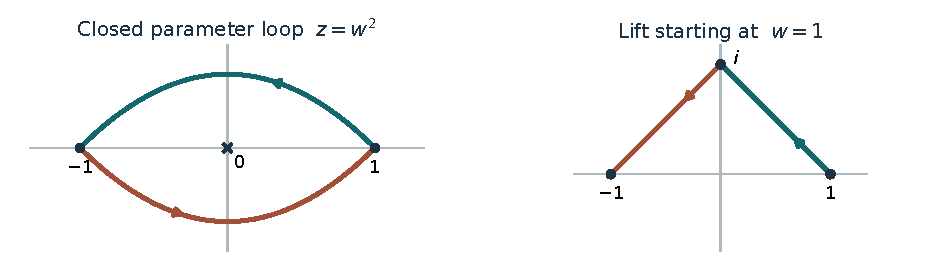
\includegraphics[width=.87\linewidth]{figures/square_root_lift.pdf}
\caption{Each color denotes one half of the parameter interval. The squared path closes at $1$. Its lift ends at $-1$ and therefore cannot give a section over the closed loop.}
\label{fig:lift}
\end{figure}
Suppose a root $y(t)$ along this loop is supplied at dyadic times by regular complex names, with a modulus ensuring that sufficiently close times give values at distance $\le1/4$. At each sampled time at least one of $|y-w|,|y+w|$ exceeds $1/2$, since their sum is at least $2|w|\ge\sqrt2$. Comparing approximations with sufficiently small fixed error (say $1/32$) identifies a factor with norm provably greater than $1/4$. In $(y-w)(y+w)=0$ this factor is invertible with an explicit norm lower bound, so the other is zero. This gives a PR sign bit at the sample, with a proof that $y$ is the indicated root; an input name here is a fixed PR family or a finite-demand parameter as specified in the framework. Choose a uniform dyadic grid whose mesh is at most $1/16$ and is within the supplied modulus at tolerance $1/4$. The path $w$ is $3$-Lipschitz, so adjacent $w$'s differ by $<1/4$. Opposite bits at adjacent samples $j,j+1$ would imply
\[
  2|w_j|\le |w_j+w_{j+1}|+|w_j-w_{j+1}|
            = |y_j-y_{j+1}|+|w_j-w_{j+1}|\le1/2.
\]
Thus adjacent bits agree. Induction is on bit equality with the first bit, and uses no unbounded extensional equality of complex names as its induction predicate. At the two endpoints the bit is the same and $w$ has changed sign, so $y(1)=-y(0)$, whereas $y(0)^2=1$. A periodic root label is impossible. This example distinguishes the existence of local analytic sheets with explicit separation from their compatibility on a loop. The finite test applies to a general analytic family once the charts and overlap transports have been justified. It does not derive those charts for arbitrary computable coefficients.

\subsection{Effective stable images in inverse towers}
\label{sec:stable-image}
The repository's categorical descent report exhibits a tower with PR-inhabited levels and no computable coherent point, and gives a construction when every bonding map is surjective. There is a useful intermediate hypothesis for towers with dead ends.

Let $A_n=\{x<b(n):V(n,x)=1\}$ be a fixed PR table family and $p_n:A_{n+1}\to A_n$ a fixed PR family of maps with a proof of typing. For $m\ge n$, let $p_{n,m}$ be the composite down from level $m$, with $p_{n,n}=1$. Suppose $h$ is a specified nondecreasing PR function with $h(n)\ge n$. Compute by bounded image search
\[
       I_n=p_{n,h(n)}(A_{h(n)}).
\]
Write $J(n,m)=p_{n,m}(A_m)$ and let $C(n)$ be the finite equality $p_n(I_{n+1})=I_n$. Given the inputs for a particular $n$, $C(n)$ is decidable by a PR test.

\begin{theorem}[Testing a proposed stable-image horizon]\label{thm:stable}
Under the preceding conditions, iPRA proves the equivalence
\[
 (\forall n\, C(n))\quad\longleftrightarrow\quad
 (\forall n\,\forall m\ge h(n)\; J(n,m)=I_n).
\]
If these conditions hold, there is a fixed PR producer which, given $a\in I_n$, extends $a$ to an infinite coherent tail in the sense of a PR function of $n,a,k$ returning its element at level $n+k$. In particular any member of $A_{h(0)}$ gives a coherent point.
\end{theorem}

\begin{proof}
Images decrease as the horizon increases by associativity of composition and typing. Stability at all horizons gives
\[
 p_n(I_{n+1})=J(n,h(n+1))=I_n
\]
because $h(n+1)\ge h(n)$. Conversely take $a\in I_n$. For $x\in I_j$ choose the first $y<b(j+1)$ with $y\in I_{j+1}$ and $p_j(y)=x$. This bounded scan has a default, ruled out on valid inputs by $C(j)$. Starting at $a$ iterate it by primitive recursion for $k$ steps, obtaining $x_k$. With $n,a$ as parameters, the invariant $x_k\in I_{n+k}$ and $p_{n,n+k}(x_k)=a$ is a pair of bounded numerical tests. The one-step equation and the composition law for $p$ preserve it. Local coherence follows at each $k$ from the scan. For $m\ge h(n)$ take $k=m-n$. This produces an $A_m$ preimage of $a$, whereas decreasing images give the reverse inclusion. Finally $p_{0,h(0)}$ maps any supplied element of $A_{h(0)}$ to $I_0$. This also specifies every PR definition and induction instance needed for the tail producer.
\end{proof}

For an example with nonsurjective bonding maps take $A_n=[3]$, with every bonding map fixing 0 and 1 and sending 2 to 1. Then $h(n)=n+1$ works, and the full bonding maps all miss 2. The restricted system has two coherent points. Using a proposed horizon requires a proof of its uniform validity.

In fact finite cardinalities alone cannot compute a valid horizon. Given machine index $e$, put $A_n=[2]$, and let $p_n$ be the identity except when the machine first halts at step $n$ on its designated input, in which case $p_n$ is constant zero. Bounded simulation gives a uniformly PR family. Externally each such tower has an eventually stable image at every level and even a coherent all-zero point. If a uniform algorithm returned a valid $h(0)$, then $J(0,h(0))$ would be the eventual image at zero. Compute this finite image. Its size is one exactly when the machine eventually halts, otherwise two. This would decide halting. This metatheoretic obstruction concerns production of horizons, even in examples where producing one coherent branch is trivial.

\paragraph{Lean dependency order.}
The checked file \texttt{lean/Forest.lean} realizes the path calculation and the inverse maps on morphisms over one connected component. Its parameter \texttt{Chart} supplies the selected paths and the empty-path equation at the root. Its edge set may contain both signs of each generator. \texttt{extend\_restrict} and \texttt{restrict\_extend} use pointwise equality.
The separate file \texttt{lean/ForestObject.lean} imports \texttt{ConciseIPRA.PR}. Its theorem \texttt{liftEdgeImp} constructs an actual arithmetic derivation of one naturality square from three local equations, namely $T_s^A(T_s^A)^{-1}x=x$, intertwining at $(T_s^A)^{-1}x$, and $T_t^B(T_t^B)^{-1}y=y$ at the indicated target value. The maps are object-language terms with one input and arbitrary shared numerical parameters.

To complete the numerical forest theorem, encode a graph as vertex and edge bounds, two endpoint arrays and an array of pairs of signed words. Encode a system by the fibre bounds and pairs of inverse tables. Implement the marking recursion and check the two bounded component invariants together with the decrease of parent times. This yields the selected paths and the root equation used in \texttt{Forest.lean}. Prove the transport of a reversed path is the inverse table, entrywise by induction on the word prefix. Induct on prefixes of a rooted forest path for the equation $h_vT_v^A=T_v^Bh_r$ and for the telescoping identity. Then use \texttt{liftEdgeImp} for each requested edge and entry. A bounded conjunction over all entries gives naturality of the extended table. Filtering the root table codes by \eqref{eq:intertwine} and ranking the retained tables then gives exactly the requested morphism list. For the tower theorem, first derive the concatenation equation for $p_{n,m}$ by induction at a fixed input. Encode $I_n(x)$ by a bounded disjunction over $u<b(h(n))$ with $V(h(n),u)=1$ and $p_{n,h(n)}(u)=x$. The same bounded-scan lemma gives the first lift, to which the invariant in Theorem~\ref{thm:stable} applies. These remaining numerical inductions are specified human proofs.

\section{Recovering inverse moduli from polyhedral data}\label{sec:pairpoly}

An embedding comes with a particularly expensive input in the repository's quantitative Jordan theorem. For a circle parametrization $f$, its inverse modulus $V$ must turn $d(s,t)\ge 2^{-k}$ into $\|f(s)-f(t)\|_\infty\ge 2^{-V(k)}$. The dimension-invariance packet also needs inverse separation, there at a specified scale. A finite table of rational affine pieces already contains this information. We extract it, including an exact best constant and an attaining pair. When the table describes a self-intersection the same calculation finds the intersection parameters.

\paragraph{Representations.}
A cell in $\mathbb Q^D$ is a bounded intersection of a finite list of closed rational affine half-spaces $h_i(z)\ge0$. Include an explicit bounding box among its rows. Equalities are pairs of rows. A pair of source points has a finite cover by such cells, on each of which two nonnegative quantities are affine:
\[
     l(z)=d(x,y),\qquad m(z)=d'(f(x),f(y)).
\]
The coordinates $z$ encode $(x,y)$ within that cell. Values agree on overlaps, and $l=0$ implies $m=0$. These are presentation conditions. In the two constructions below the coverage, value compatibility and box come directly from the input. A generic atlas used as input must supply those conditions. All finite operations below are on rational codes.

For example, on a bounded union of rational simplexes take a continuous piecewise affine map given by its vertex values, with compatible values on shared faces. Use a simplex pair with two vectors of barycentric coordinates as variables. Require each vector to be nonnegative and to sum to one. Both points and their images are affine in these coordinates. The input and output maximum norms are each the maximum of a finite list of signed affine coordinate differences. For each choice of an entry in each list, append comparisons making those entries maximal. Enumerating the choices covers all pairs, including ties. Assume a valid geometric presentation, so two barycentric descriptions of one source point give the same image. The same construction works for a domain consisting of one simplex and for triangulated cubes.

For a polygonal circle let $0=b_0<b_1<\cdots<b_N=1$ be rational breakpoints. Give $P_i\in\mathbb Q^m$ for $0\le i\le N$ with $P_N=P_0$, $m\ge1$. On $[b_i,b_{i+1}]$ use affine interpolation. Symmetry allows $s\le t$. In each rectangle of parameter intervals impose that order and split it by $t-s=1/2$. The two formulas for $l$ are $t-s$ and $1-t+s$. For each possible signed output coordinate impose that it dominate all the others and use it for $m$. Thus $D=2$ independent of the number of edges and target dimension. The pair $(0,1)$ denotes one circle point and gives $l=m=0$.

\begin{lemma}[Finite vertex interpolation]\label{lem:pairvertex}
For a cell $H$, enumerate all choices of $D$ rows, solve their equality systems with nonzero determinant, and retain solutions satisfying every row. Every rational $z\in H$ has a primitive recursively constructed binary tree of convex combinations of retained points, of depth at most $D$. Duplicate retained points do no harm.
\end{lemma}
\begin{proof}
At $z$ mark a row active when $h_i(z)=0$. Compute the rank $r$ of the active linear parts by scanning nonzero minors (the empty minor is one). If $r=D$, the independent active rows yield $z$ by Cramer's rule, so this point is on the list. Otherwise choose a nonzero rational vector $w$ annihilated by all active rows. Explicitly choose an $r$-by-$r$ invertible row-column submatrix, set one free coordinate to one and the other free coordinates to zero, and solve its $r$ equations for the pivot coordinates. Every remaining active row is in the span of the pivot rows: after their elimination any nonzero free entry would give a nonzero $(r+1)$-minor. This also covers $r=0$.

Along $z+tw$ an inactive row has positive slack $h_i(z)$ and directional slope $a_i\cdot w$, where $a_i$ is its linear part. Among negative slopes take the least positive $h_i(z)/(-a_i\cdot w)$ to get $t_+$. Along $-w$ obtain $t_-$ by the same rule. A nonzero coordinate of $w$ and its two box rows ensure both lists are inhabited. An active box face would force that coordinate of $w$ to vanish. The two endpoints $z^+=z+t_+w$ and $z^-=z-t_-w$ satisfy every row, retain all old active rows and activate a new row with nonzero slope on $w$. Such a row is independent of the old rows. Their convex combination with respective weights $t_-/(t_-+t_+)$ and $t_+/(t_-+t_+)$ is $z$. In a depth-$D$ tree split unmarked nodes in this way, padding finished leaves by their own copies if desired. Along every branch the active rank increases at each genuine split, so the leaves belong to the enumerated list. Substitution proves the convex-combination identity at every node. All minima used here are over explicit row lists.
\end{proof}

\begin{theorem}[Sharp distortion or a rational collision]\label{thm:pairratio}
Suppose at least one pair has positive source distance. On all retained points in all pair cells with $l(v)>0$, compute
\[
       c=\min_v\frac{m(v)}{l(v)},\qquad L=\max_v\frac{m(v)}{l(v)}.
\]
Then $c\,d(x,y)\le d'(f(x),f(y))\le L\,d(x,y)$ for every rational pair, and both bounds are attained at rational pairs of positive source distance. If $c=0$ the attaining pair is a collision. If $c>0$ it gives quantitative injectivity. If there is no positive-distance pair, the scan is empty and every distance is zero.
\end{theorem}
\begin{proof}
A positive $l(z)$ is a convex combination of nonnegative leaf values, hence some leaf has positive $l$. The scan is inhabited. The inequalities hold at each retained point of positive $l$ by the two comparisons in the scan. At every retained point of zero $l$, the consistency condition gives $m=0$. Thus no division on the diagonal is required. On each cell both inequalities are affine inequalities. Propagate them up the tree by multiplying each inequality by its nonnegative weight and adding. The result at the root holds for the specified pair. As every retained point is feasible, the two winning pairs are genuine and realize the two ratios. A positive-distance collision forces $c=0$ by the lower bound. For named pairs the same inequalities follow at each requested precision by rational approximation, since both metrics and the specified continuous PL functions respect limits. In the rational PL constructions the upper bound provides an explicit continuity rate for this last passage.
\end{proof}

\paragraph{Discharging the repository hypotheses.}
Write the positive $c=a/b$ and $L=p/q$ with positive denominators. Take $j_-$ least with $2^{j_-}a\ge b$, scanning through $b$, and $j_+$ least with $2^{j_+}q\ge p$, scanning through $p$. The inequalities $2^b\ge b$ and $2^p\ge p$ justify the budgets. For the Jordan packet take
\[
      V(k)=k+\max(8,j_-),\qquad U(k)=k+\max(8,j_+).
\]
The rational evaluator is simply affine interpolation on the first interval containing the parameter. The inequalities of the theorem imply both modulus premises in the packet at rational parameters, even before its allowance for two approximation errors. For a PL cube the dimension-invariance packet asks that an image discrepancy (including evaluation error) below $2^{-a_0}$ imply source distance at most $1/2$. Take $a_0=1+j_-$. An actual image discrepancy below $2^{-a_0}\le c/2$ forces $d(x,y)<1/2$ by the lower bound. The extra nonnegative evaluation-error term in that packet preserves the implication for the exact rational evaluator. A crossing circle returns explicit unequal parameters instead. This supplies numerical regularity data to the existing mathematical proofs. Their remaining parity and incidence derivations in Lean are separate obligations.

\paragraph{Two examples and a perturbation.}
Traverse the unit square in four equal parameter intervals. Its exact $(c,L)$ is $(2,4)$. On one edge the ratio is $4$; on adjacent edges let the two distances to the shared vertex be $a,b$ in edge-length units. The shorter parameter distance is at most $(a+b)/4$, and the image distance is $\max(a,b)$. On opposite edges the image distance is at least one and the parameter distance is at most $1/2$. The opposite vertices attain ratio two. Traversing the bow-tie $(0,0),(1,1),(0,1),(1,0),(0,0)$ in the same intervals gives $c=0$ at $s=1/8$, $t=5/8$. If a map $g=P+R$ satisfies $\|R(s)-R(t)\|_\infty\le e\, d(s,t)$, the triangle inequality gives lower and upper constants $c-e$ and $L+e$ for $g$. For a curved example use the square and $R(s)=(s(1-s),0)$. For $s\le t$ the factorization of the difference gives $|R_1(t)-R_1(s)|\le t-s$. Applying the same bound on the two endpoint intervals and $R(0)=R(1)$ also gives $1-t+s$. Thus $e=1$ and the curved circle has bounds $(1,5)$, with fully rational evaluation at rational parameters.

\paragraph{A version for uniform approximation.}
Suppose a polygon $P$ is uniformly within $e$ of a curve at the current demand $k$. Intersect its pair cells with the single new half-space $l\ge 2^{-k}$. Minimize the affine image distance over the retained vertices, obtaining $h$. If these cells are empty, the separation condition at this scale is vacuous by Lemma~\ref{lem:pairvertex}. Otherwise every eligible image pair of the curve is separated by at least $h-2e$, by the triangle inequality. A check $h>2e$ now produces the inverse exponent by the same finite denominator bound as above. This test can succeed even if $P$ crosses itself at a smaller parameter separation. A PR choice of such table and error for each $k$, with checks passing, suffices for a uniform inverse modulus (take prefix maxima and pad). A failed test establishes only that this particular estimate is insufficient.

\begin{proposition}[Why a forward modulus alone gives no uniform PR extraction]\label{prop:delayedcurves}
There is a single PR evaluation scheme for a family of embedded circles with a common forward Lipschitz bound for which no PR function of the family index supplies even $V(1)$ uniformly. This is an external assertion about the standard natural numbers.
\end{proposition}
\begin{proof}
Enumerate all syntactic unary PR definitions, treating invalid codes as the zero function. An ordinary machine $M(e)$ evaluates definition $e$ on $e$ and then spends more than the result in additional steps. For each standard $e$ the computation terminates: evaluate compositions by their constituents and recursion by a finite loop. Let its running time be $T(e)$. For any unary PR function $g$ take an index $e$ of $g$; then $T(e)>g(e)$.

Let $P$ be the unit-square circle above and set $f_e(s)=2^{-T(e)}P(s)$. At demand $n$ run exactly $n$ steps of the machine simulation. If it halted, its time is available and the evaluator returns $2^{-T(e)}P(s)$. Otherwise return the zero vector. The bounded simulation is PR. The uniform error is at most $2^{-n}$, since $\|P\|_\infty\le1$. Each curve is a positive multiple of an embedding and all have forward Lipschitz bound 4. Opposite vertices at parameters $0$ and $1/2$ have distance exactly $2^{-T(e)}$. An inverse exponent $g(e)$ at $k=1$ therefore satisfies $g(e)\ge T(e)$ for every $e$, contradicting the preceding diagonal argument. The example concerns uniformity over presentations; each fixed index has a valid numerical modulus. It makes no claim that iPRA proves termination of $M$ uniformly. The vertex algorithm instead accepts the actual rational PL table, whose denominators contain the missing quantitative information.
\end{proof}

\paragraph{Arithmetic and Lean obligations.}
The PR loops enumerate row subsets (bit masks below $2^H$ for $H$ rows), column subsets and permutations for determinants. Cramer's rule uses rational products and bounded comparison, with zero divisors tested first. Rank uses a finite maximum. For the interpolation proof use the complete binary tree of depth $D$, with at most $2^{D+1}-1$ positions. At level $a$ the invariant is the conjunction over its node indices that each point is feasible and its rank is at least $\min(a,D)$; finished vertices can be repeated. Additional conjuncts check each parent interpolation identity and the nonnegative rational weights. At a node the row tests, minor scans, determinant expansion and endpoint computations are finite identities or comparisons; determinant row elimination follows by multilinearity and alternating cancellation of the bounded permutation sum. The rank-growth check can also be proved by adjoining the new row to the pivot submatrix: eliminating the old pivot columns of that row leaves a nonzero free entry, since it has nonzero dot product with $w$. Backwards level induction on the bounded conjunction of the two affine inequalities propagates the leaf bounds. Node states are PR functions of the input and level, so even enormous intermediate numerators do not introduce an unbounded existential in the invariant. The chart and queried rational pair stay fixed during these inductions. The resulting universal closure over numerical codes and the two alternative numerical outputs are legitimate iPRA targets. There is no induction on a statement quantifying over all convex sets or real vectors.

The executable \texttt{checks/polygon\_modulus.py} implements the two-variable algorithm. It checks both extrema by independent interpolation for eight examples, including crossing, retraced and constant maps. In \texttt{lean/PairBounds.lean}, \texttt{Mix} is the inductively defined list-vertex/convex-split relation on rational pairs $(l,m)$. The checked lemma \texttt{lower\_of\_mix} propagates a finite Boolean lower-bound test through a supplied tree. The upper inequality follows by carrying $L l-m\ge0$ through the same affine-combination rule. The file also checks sharpness at an attained pair and the two perturbation inequalities. The actual object-language file \texttt{lean/PairBoundsIPRA.lean} proves \texttt{closed\_mix\_lower}. Its matrix is
\[
 Au\le BU\ \longrightarrow\ Av\le BV\ \longrightarrow\
 A(ru+sv)\le B(rU+sV)
\]
with all eight number variables universally closed. Clearing denominators in one convex split gives exactly this implication, because distances and weights are nonnegative. For the upper bound exchange the two distances and the two slope factors. To finish the full \texttt{Prf PRAAx} endpoint, implement the row, determinant and tree computations as fixed PR symbols, prove the rank/active-row invariant above, apply this split rule level by level and reflect the bounded argmin and argmax checks. The closed split rule is a checked object derivation. The rational host lemmas, constructive interpolation proof and numerical runs have the individual scopes stated here.

\section{Constructing a path around the parameter poles}\label{sec:detours}

The nonresonant connection theorem in the repository asks for a parameter-continuation chain avoiding poles and resonance \cite{hyper}. The forbidden values include entire integer translates of hyperplanes, so a path in the real parameter space need not exist. In the complex parameter space we can compute a polygon with a uniform positive clearance. The result is independent of the special functions to be transported along it.

\begin{theorem}[Five-segment detour]\label{thm:detour}
Let $\ell_j(z)=b_j+u_j\cdot z$ ($1\le j\le J$) be nonconstant affine forms with real rational coefficients on $\mathbb C^d$. For each form prescribe $S_j=\mathbb Z$, $\mathbb Z_{\le0}$ or $\{0\}$. From Gaussian rational endpoints $x,y$ satisfying $\ell_j(x),\ell_j(y)\notin S_j$, a PR algorithm produces at most five rational line segments from $x$ to $y$ and a positive rational $\gamma$ such that at every point of the polygon
\[
 \max\{|\Re\ell_j(z)-n|,|\Im\ell_j(z)|\}\ge\gamma
 \quad(j\le J,\ n\in S_j).
\]
It also produces a subdivision and overlapping parameter boxes on which half the clearance persists. The dimension, forms and number of families are allowed to vary as input data.
\end{theorem}

\begin{proof}
Use the maximum of the absolute values of all real and imaginary coordinates as the parameter norm. Empty families allow the straight segment with any positive clearance. Assume $J>0$. First find an integer vector $v$ on which every $u_j$ is nonzero. Clear each row's denominators, write its integer coefficients as $a_{ji}$ indexed from zero, and take
\[
 T=2+\max_j\sum_i|a_{ji}|,\qquad v=(1,T,\ldots,T^{d-1}).
\]
In a row of degree $h>0$ the leading term has magnitude at least $T^h$, whereas the sum of the magnitudes of the lower terms is at most $(T-2)T^{h-1}<T^h$. Degree zero is immediate. One may scan smaller positive integers first and select the first passing the same nonzero tests. Use the \emph{original} rational rows to set
\[
 s_j=u_j\cdot v,\qquad A=\max(1,\max_j|s_j|),\qquad m=\min_j|s_j|>0 .
\]

For $p=x,y$ let $q_j=\Re\ell_j(p)$ and let $\rho_{jp}$ be the exact maximum-norm distance of $\ell_j(p)$ from $S_j$. Compute it as the maximum of $|\Im\ell_j(p)|$ and the real distance from $q_j$ to $S_j$. The latter uses just floor and ceiling, with the candidates clipped at zero for the nonpositive ray. For a singleton it is $|q_j|$. Let $\eta_p$ be the minimum of $1$, the positive $\rho_{jp}$ and the distances of all \emph{nonintegral} $q_j$ to $\mathbb Z$; discard integral $q_j$ only in this last list. It follows that $\eta_p>0$. Set $\delta_p=\eta_p/(4A)$. The six vertices of the polygon are
\[
 \begin{gathered}
 x,\qquad x+\delta_xv,\qquad \Re x+\delta_xv+i v,\\
 \Re y+\delta_yv+i v,\qquad y+\delta_y v,\qquad y .
 \end{gathered}
\]
On the two short end segments the value of every form varies by at most $\eta_p/4$ from its endpoint, so its distance to its forbidden set remains at least $3\eta_p/4$. At the shifted real part $q_j+\delta_p s_j$, a nonintegral $q_j$ still has distance at least $3\eta_p/4$ from every integer. An integral $q_j$ has moved by a nonzero amount at most $1/4$, so its new distance to the integers is $\delta_p|s_j|\ge\delta_pm$. On each vertical segment that real part stays fixed. The middle segment has fixed imaginary vector $v$, so the imaginary part of every form has magnitude at least $m$. Consequently a valid choice is
\[
 \gamma=\min\{3\eta_x/4,\,3\eta_y/4,\,\delta_xm,\,\delta_ym,\,m\}.
\]
This argument covers allowed integral real values of gamma arguments as well as nonreal endpoints whose real part is a forbidden integer.

Put $B=\max(1,\max_j\sum_i |u_{ji}|)$ and $r=\gamma/(4B)$. On a closed coordinate box of radius $2r$ around a polygon point, each form moves by at most $2Br=\gamma/2$. Subdivide an edge of norm length $b$ into $\max(1,\lceil b/r\rceil)$ equal intervals. Successive centers are at distance at most $r$, and their $2r$ boxes have an overlap with positive width. All coordinates, counts and bounds are rational or integral. For the arithmetic assertion fix a rational position on a segment and an arbitrary signed integer $n$ in the permitted set. The inequalities above give the desired result without enumerating infinitely many parallel hyperplanes. Generalize over the position and $n$ after the bounded computations. On named positions the same bound follows at every precision by affine evaluation and the rational-gap argument.
\end{proof}

\paragraph{Named endpoints.}
If $x,y$ have fixed PR regular names instead, supply lower bounds $\beta_p>0$ on all the endpoint distances. Sample each endpoint to norm error at most $\beta_p/(8B)$. For regular names the approximation to the represented point has the specified error at its working precision; equivalently use finer pairs and their regularity inequalities. The resulting rational endpoint has clearance at least $7\beta_p/8$. The segment connecting the endpoint to its approximant stays within $\beta_p/(8B)$ of the original endpoint. Attach these two segments to the rational polygon, taking the minimum of the clearance bounds. This avoids deciding whether a real part given by a name is an integer. A certificate of mere nonequality at an unnamed point does not supply the required margin.

\paragraph{Gauss's connection at one.}
In the standard nonresonant two-term formula let $d_0=c-a-b$. The coefficients have the forms
\[
 \frac{\Gamma(c)\Gamma(d_0)}{\Gamma(c-a)\Gamma(c-b)},\qquad
 \frac{\Gamma(c)\Gamma(-d_0)}{\Gamma(a)\Gamma(b)} .
\]
Use the five forms $c,c-a,c-b,a,b$ with $S=\mathbb Z_{\le0}$ and the form $d_0$ with $S=\mathbb Z$. The last guard also excludes the denominator singularities of the two local series at $1$, whose lower parameters are $1\pm d_0$. All normals are rational. Starting chambers can be represented, for example, by $a=1/4,b=1/3,c=5/4$ (positive $d_0$) and $a=1/2,b=2/3,c=1$ (negative $d_0$), satisfying the indicated gamma guards. The theorem connects either point to every admissible Gaussian rational triple and returns radii and a finite overlap chain. This discharges the \emph{geometric path and clearance} part of item 3 of the repository theorem on that parameter domain. It applies as well to any additional finite list of real-rational affine pole families with the same form of guard if the endpoints pass their tests. The analytic identities and parameter-jet estimates needed to propagate the gamma evaluation through those boxes are distinct obligations. To continue an identity in the parameters one needs matching parameter jets, for instance from an identity valid on an initial open chamber. Equality at a single starting triple does not determine a holomorphic function of three parameters. For the integer resonances excluded here, Section~\ref{sec:resonance} constructs a basis directly.

\paragraph{One crossing in parameter space.}
Fix $a=1/4,b=1/3$, and vary only $c$ between $5/4$ and $1/2$. A real segment crosses $c=a+b=7/12$. In dimension one take $v=1$ and omit the already checked constant forms $a,b$. The normal slopes of the remaining four forms are one. Both endpoints satisfy the hypotheses, although $c-a$ at the first one is the allowed integer $1$. The executable certificate computes the polygon and verifies the clearance on \emph{whole} segments using independent rational minimization. This example crosses between nonresonant chambers; it prescribes no traversal through the resonant point.
Concretely the four interior vertices are $61/48$, $61/48+i$, $25/48+i$, $25/48$. The certificate gives $\gamma=1/48$, a subdivision scale of $1/192$, and interval counts $4,192,144,192,4$. The checks in \texttt{Detour.lean} cover the single-form clearance inequalities along all three kinds of segment.

\section{Resonance at a regular singular point}
\label{sec:resonance}

The hypergeometric packet constructs a nonresonant connection formula. Its
remark on resonant connection formulas leaves a uniform treatment of integral
exponent differences open. Two gamma terms can each diverge in a parameter
limit, even when their sum has a well-behaved logarithmic expansion. We
construct the two local solutions directly. The classical comparison is
NIST DLMF, \S15.10(i), equations (15.10.8)--(15.10.10) and part (d);
the construction below supplies uniform numerical bounds for the
iPRA interpretation.\footnote{\url{https://dlmf.nist.gov/15.10.i}}
The same finite operation works
whenever a known solution is a monomial times a power-series unit and the
Wronskian has that form as well.

Write $K=\mathbb Q(i)$ and $|x+iy|_1=|x|+|y|$. We use $|\cdot|_1$ for
all the estimates below. A coefficient array is computed only through its
requested degree. Products of arrays use truncated convolution. For
$J\ge0$ and $R>0$ put
\[
  \|v\|_{J,R}=\sum_{j=0}^J |v_j|_1R^j .
\]
Truncated convolution has norm at most the product of the two norms: expand
the two nonnegative sums and retain the pairs with index sum at most $J$.

\begin{lemma}[Primitive of a Laurent series with one finite principal part]
\label{lem:res-primitive}
Suppose every prefix of $g$ has $\|g\|_{J,R}\le M$. For $k\in\mathbb N$,
the expression
\[
 H(t)=g_k\log t+
 \sum_{\substack{j\ge0\\j\ne k}}
       \frac{g_j}{j-k}t^{j-k}
\]
gives a primitive of $t^{-k-1}g(t)$ on a named logarithm chart with
$0<|t|_1\le R/2$. Keeping $j\le k+N$ gives error at most
$MR^{-k}2^{-N-1}$. The logarithm is part of the exact expression even at
cutoff $N=0$.
\end{lemma}
\begin{proof}
Every omitted exponent is positive. For every subsequent finite tail,
multiply and divide its terms by $R^j$, use $1/(j-k)\le1$, and bound
$(|t|_1/R)^{j-k}$ by $2^{-N-1}$. The resulting bound is independent of
the second cutoff. Formal differentiation sends the exceptional summand to
$g_k/t$, and sends every other summand to $g_jt^{j-k-1}$. At a requested
point the negative powers are finite and require a supplied apartness
bound. Derivatives of the positive tail converge with explicit clocks too:
the $d$th derivative, $d=1,2$, costs a factor at most
$R^{-d}2^d(j-k)^d$ against the bound $R^{-k}2^{-(j-k)}$ for
$j-k\ge d$. The elementary bound $n^2\le 64\,2^{\lfloor n/2\rfloor}$
for $n\ge1$ follows by checking $1\le n\le8$ and stepping by two.
Thus twice the requested bit precision plus an integer offset for the
displayed constants suffices. Termwise differentiation here can equivalently
be read as a finite Taylor estimate: for polynomials expand
$(t+h)^n-t^n-n t^{n-1}h$ by the binomial identity and bound the remainder
by $n(n-1)|h|_1^2(|t|_1+|h|_1)^{n-2}/2$. On a slightly larger disk
(e.g. $3R/4$) the weighted derivative tails still decay geometrically
(group four powers to use $(3/4)^4<1/2$). The rational inequalities pass
to names at any prescribed precision.
\end{proof}

\subsection{A basis uniform in the signed exponent difference}

Fix Gaussian rationals $a,b,c$ and a signed integer $m=c-a-b$. Use
$t=1-z$, $k=|m|$, $s=\min(0,m)$ and $r=\max(0,m)$. The following formulas
also work when upper parameters terminate. Let $h_0=B_0=u_0=1$, and set
\[
\begin{aligned}
 h_{j+1}&=h_j\frac{(a+r+j)(b+r+j)}{(j+1)(j+1+k)},&
 B_{j+1}&=B_j\frac{c+j}{j+1},\\
 u_n&=-\sum_{j=1}^n h_j u_{n-j}\quad(n>0),&
 g&=B*u*u .
\end{aligned}
\]
Here $B$ is the series for $(1-t)^{-c}$ at zero. This notation can be
defined by its displayed recurrence, equivalently by $(1-t)B'=cB$ and
$B(0)=1$. Use the rational radius
\[
 R=\big[4\max\{1,(1+|a+r|_1)(1+|b+r|_1),1+|c|_1\}\big]^{-1}.
\]

\begin{theorem}[Local resonant solutions and logarithmic coefficient]
\label{thm:res-gauss}
On $0<|t|_1\le R/2$ with a specified logarithm branch, a fundamental pair
for Gauss's equation in the coordinate $t$ is
\[
 U=t^r h(t),\qquad V=U H(t),
 \qquad U V'-U' V=t^{m-1} B(t),
\]
where $H$ is given by Lemma~\ref{lem:res-primitive}. All coefficient and
tail algorithms are uniform primitive recursive functions of the rational
parameters, the signed resonance and the requested precision, with the
point and branch guards described below. With $(x)_k=\prod_{j<k}(x+j)$
and $(x)_0=1$, the logarithmic coefficient in $H$ is
\[
 \boxed{\displaystyle
 g_k=\frac{(-1)^k(a+s)_k(b+s)_k}{(k!)^2}.}
\]
Consequently a change of logarithm by $2\pi i$ sends $V$ to
$V+2\pi i g_k U$. For rational parameters this also decides exactly when
the logarithmic term disappears.
\end{theorem}

\begin{proof}
A substitution in the equation gives
\[
 L y=t(1-t)y''+[1-m-(a+b+1)t]y'-aby=0 .
\]
Inserting $t^e v(t)$ and dividing by $t^e$ contributes a term
$e(e-m)v/t$. For $e=r$ or $s$ this vanishes. The resulting Gauss operator
has upper parameters $a+e,b+e$ and derivative constant $1-m+2e$.
For $e=r$ this constant is $1+k$. Coefficient comparison gives exactly
the recurrence for $h$ above, hence $LU=0$.

For every prefix the coefficient ratios bound
$|h_j|_1 R^j, |B_j|_1 R^j\le 4^{-j}$. For example
$|a+r+j|_1\le(1+|a+r|_1)(j+1)$, and the denominator in the recurrence
for $h$ is at least $(j+1)^2$. Therefore $\|h-1\|_{J,R}\le1/3$.
In the algebra of polynomials modulo $t^{J+1}$,
$u=\sum_{d=0}^{J}(1-h)^d$, since the error term has degree at least
$J+1$. This proves the displayed inverse recurrence,
$\|u\|_{J,R}\le3/2$ and $\|g\|_{J,R}\le(4/3)(3/2)^2=3$.
Replacing $c$ by $-c$ gives an array $B_{-c}$ with the same bound
$4/3$. The formal derivative of $B B_{-c}$ is zero and its constant is
one, by the first-order equations and cancellation of $1-t$ in truncated
coefficient calculations. Thus $B^{-1}=B_{-c}$.

In the normalized ODE the coefficient of $y'$ is
$p=(1-m)/t-c/(1-t)$. Consequently $W=t^{m-1}B$ satisfies $W'=-pW$.
From $r-s=k$ and $r+s=m$ we get $W/U^2=t^{-k-1}g$. Defining
$V=UH$ gives $UV'-U'V=U^2 H'=W$. Differentiating this equation gives
$U(V''+pV'+qV)=0$ because $U''+pU'+qU=0$, where
$q=-ab/[t(1-t)]$. Multiplication by $t^{-r}u$ cancels $U$.
The inverse determinant has the explicit name $t^{1-m}B_{-c}$. This
constructs a fundamental matrix with an inverse, even if $g_k=0$.
For any solution germ presented by a convergent Taylor expansion at an
ordinary point, multiplying its initial jet by this inverse gives its
unique two coordinates. The jet uniqueness and transport estimates below
prove equality of the resulting solutions throughout any specified chain
of overlapping charts.

It remains to identify the logarithm. If $k=0$, $g_0=1$. For $k>0$, write
$t^{-s}V=Q+g_k t^k h\log t$. Here $Q$ is an ordinary power series, since
$t^k$ cancels the finite principal part, and $Q_0=-1/k$.
Put $A=a+s$, $D=b+s$. The transformed equation has derivative constant
$1-k$. Applying its operator to $t^k h\log t$, the logarithmic part
vanishes. The remainder is
$2(1-t)(t^k h)' +[-k/t-(A+D)]t^k h$, whose first term of degree $k-1$
has coefficient $k$. For $1\le j<k$ coefficient comparison at $j-1$ now
gives
\[
 j(j-k)Q_j=(A+j-1)(D+j-1)Q_{j-1}.
\]
At $j=k$ the coefficient of $Q_k$ is zero and
$kg_k=(A+k-1)(D+k-1)Q_{k-1}$. Multiply the first $k-1$ recurrences,
using $\prod_{j=1}^{k-1}j(j-k)=(-1)^{k-1}((k-1)!)^2$.
Iteration uses division only by the nonzero integers $j(j-k)$, including
when an upper rising factorial vanishes. This proves the boxed identity.
Changing only the logarithm in $H$ gives the asserted shear.
\end{proof}

\paragraph{Precision data.}
The finite negative-power sum uses rational arithmetic at Gaussian-rational
points. At named points, a lower bound $|t|_1\ge\delta>0$ gives
$|1/t|_1\le 2/\delta$, since $(|x|+|y|)^2\le 2(x^2+y^2)$.
For a branch supply an evaluation procedure for $\log t$ with its error
clock and a bound on its norm. A chart based at $x$ translates by
$\log(x+u)=\log x+\sum_{j\ge1}(-1)^{j+1}(u/x)^j/j$ for $|u/x|_1<1$,
with the geometric tail from the supplied radius margin. This fixes the
derivative and the overlap convention. Positive rational $t$ has a canonical real logarithm from
$\log t=2\sum_{j\ge0} v^{2j+1}/(2j+1)$, $v=(t-1)/(t+1)$, with tail
bounded by $2|v|^{2J+1}/(1-|v|^2)$ after $j<J$.
For the power-series tails take $M=3$ in Lemma~\ref{lem:res-primitive}.
A cutoff for accuracy $2^{-p}$ is, for example,
$N=p+\lceil 3 R^{-k}\rceil+2$ for $H$ before multiplication by $U$.
All intermediate size bounds can be propagated through finite sums and
products: if $|x|_1\le A, |y|_1\le D$ and approximants have errors
at most $\epsilon\le1$, their product error is at most
$(A+D+1)\epsilon$. This gives rational instruction-by-instruction budgets
for $U,V,U',V'$ and for the inversions above. Every induction may fix the
requested precision and a final degree $J$ first. The needed prefix
recurrences, truncated product identities, and prefix norm inequalities
are then Boolean folds on rational arrays.

\subsection{Matching the solution at zero without gamma limits}
Assume $c\notin\{0,-1,-2,\ldots\}$, a decidable condition on $K$. The
ordinary series $F(z)={}_2F_1(a,b;c;z)$ then has coefficients
$f_0=1$ and $f_{n+1}(n+c)(n+1)=f_n(n+a)(n+b)$.
Set $t_0=R/4$, $z_0=1-t_0$. Use the real logarithm at $t_0$.
With $Y=F(z_0)$, $D_0=-F'(z_0)$ and $W=UV'-U'V$, define
\[
 \alpha=(YV'-D_0 V)/W,\qquad \beta=(U D_0-U'Y)/W ,
\]
where the right sides are evaluated at $t_0$.

\begin{proposition}[Connection coefficients as rapid names]
On the overlap containing the positive interval $0<t\le R/2$,
the continuation of $F(1-t)$ from $t_0$ is $\alpha U+\beta V$, using
the logarithm continued from its real value at $t_0$ along the same
charts. The constants are uniformly PR-computable names from
$a,b,c,m$ alone.
\end{proposition}
\begin{proof}
Here is a clock even when $z_0$ is near one. Put
$E=\max(1,|a|_1,|b|_1,|c|_1)$,
$n_0=\lceil32 E/t_0\rceil$, and $q=1-t_0/2$. For $n\ge n_0$ put
$x=E/n\le 1/2$. The ratio multipliers of $f_n z_0^n$ and
$n f_n z_0^{n-1}$ both have norm at most
$z_0(1+x)^2/(1-x)$. For the derivative the factor $(n+1)/n$ cancels the
coefficient denominator $(n+1)/n$; the series itself has the smaller
bound. The reciprocal estimate follows by multiplying
$(1+c/n)^{-1}=1-(c/n)(1+c/n)^{-1}$ and taking norms. For $x\le1/2$,
$(1+x)^2/(1-x)\le1+7x$. Thus both norms are $\le q$. This argument uses
multipliers, so a vanishing term creates no division by zero. Let $M_0$ be
one plus the sum of the two term norms at $n_0$. All subsequent tails
after $N$ further terms are bounded by $M_0q^N/(1-q)$. For an explicit
loose cutoff, $q^N\le [1+N(1-q)]^{-1}$ by the finite binomial inequality.
Hence $N=\lceil 2^p M_0/(1-q)^2\rceil+1$ suffices at precision $p$.
The same inequality supplies a clock for the logarithm at $t_0$.
The previous theorem supplies the other four entries and $W^{-1}$.
Matrix multiplication gives equality of values and first derivatives
at $t_0$ exactly as names.

For completeness, agreement of jets at an ordinary point $x$ determines
the expansion there. After translation, the coefficient of the still
unknown Taylor coefficient of degree $j+2$ in the differential equation
is $(j+1)(j+2)x(1-x)$; all other terms involve earlier coefficients.
Hence the two coefficient arrays agree to every prescribed degree by
finite recurrence. Reexpansions used here exist by the binomial formula:
for a series having bounded weighted prefixes at radius $S$, expanding
$(x+u)^n$ is absolutely majorized by $(|x|_1+|u|_1)^n$. A strict gap
to $S$ gives the geometric truncation clock; locally the logarithm
translates by the Taylor series for $\log(1+u/x)$ for $|u/x|_1<1$
with its geometric tail. For the original Gauss series at a positive
point use the ratio bound above at any larger radius below one.
The Laurent powers translate by the binomial series or finite
multiplication of the local inverse. Thus on the real segment between
$t_0$ and a specified $t\in(0,R/2]$, both expansions are valid on disks
of radius $\min(t,t_0,R/4)/8$ about every segment point (for a named
$t$ use its supplied lower bound). Here are finite
bounds for the dependence on these jets. Put $d=\min(t,t_0,R/4)$
(or a positive rational lower bound), $S=d/4$, and write the differential
equation as the first-order system for $(y,y')$ with matrix
\[
 P(t)=
 \begin{pmatrix}
 0&1\\
 ab[1/t+1/(1-t)]&(m-1)/t+c/(1-t)
 \end{pmatrix}.
\]
At a segment center $x$, summing the geometric expansions of $1/t$ and
$1/(1-t)$ out to radius $S$ bounds their prefix norms by
$1/(x-S)\le 2/d$ and $1/(1-x-S)\le2$, respectively. Thus
$A=1+|ab|_1(2/d+2)+2|m-1|/d+2|c|_1$ bounds the sum of all entry norms.
Set $\rho=\min(S,1/(2A),d/8)$. For initial vector $b_0$, the recurrence
$(j+1)b_{j+1}=\sum_{i=0}^j P_i b_{j-i}$ gives
\[
 \|b\|_{J,\rho}\le |b_0|_1+\rho A\|b\|_{J-1,\rho}\le 2|b_0|_1 ,
\]
by finite induction (using the sum of coordinate norms). A transfer of
length $\le\rho/2$ has operator norm at most two, and truncating at $J$
costs at most $2|b_0|_1 2^{-J-1}$. Divide the segment into
$L=1+\lceil2|t-t_0|/\rho\rceil$ such steps. Initial errors grow by
at most $2^L$. If each transfer adds error $\epsilon$, the aggregate
added error is at most $(2^L-1)\epsilon$. Thus set
$\epsilon=2^{-p-L-2}$, and bound intermediate exact jets by
$2^L|b_0|_1$ when choosing cutoffs. These rational bounds give an
induction on errors at fixed precision in place of induction on equality
of entire analytic functions. The same jet argument extends
to specified overlap charts by finite chains with positive margins.
\end{proof}

\paragraph{Worked case.}
For $(a,b,c)=(1,1,3)$ the resonance is $m=1$,
$h=(1-t)^{-2}$ and $g=1-t$. Our basis is
$U=t/(1-t)^2$ and $V=U(-1/t-\log t)$.
The coefficients of the series at zero are $2/((n+1)(n+2))$,
so summing the partial fractions using the logarithm series gives
\[
 F(1-t)=\frac{2[(1-t)+t\log t]}{(1-t)^2}=-2U-2V .
\]
The sign of the shear and the normalization of the principal part can
both be checked on this example. For a resonance with trivial logarithm,
$(a,b,c)=(0,1,3)$ gives $k=2$ and $(a)_2=0$.

\paragraph{Formalization targets and scope.}
The repository's \texttt{HypergeometricRatio} proves cross-multiplied
identities with natural parameters. \texttt{HypergeometricOdeFormal}
already derives the Wronskian derivative in its formal differential
algebra. A Lean implementation can encode each of $h,B,u,g$ as a
degree-$J$ array of pairs of signed rationals and use the recurrences
above as bounded loops. First derive multiplication and inversion modulo
$t^{J+1}$, prefix norm submultiplicativity, and the $4^{-j}$ bounds in
the object calculus. Next encode a finite Laurent jet by a signed lower
exponent, a degree bound, and its regular and logarithmic arrays, with
$D(t^n\log t)=nt^{n-1}\log t+t^{n-1}$. To verify a coefficient of
$Ly$ through exponent $n$ request the coefficients of $y$ through $n+2$,
also allowing for the displayed monomial shifts. The boxed formula is
a rational-array recurrence with finite product invariants; the Wronskian
and basis identities reduce coefficientwise to convolution. The final
stage uses the clocks above to translate each requested identity into
rational inequalities. The included \texttt{Resonance.lean} checks six host-field
lemmas in Lean 4.32.0, including the coefficient recurrence telescope,
the exceptional-index identity and Wronskian matching. Its field
identities are reusable algebraic inputs. Encoding arrays and deriving
their norm and analytic bounds in object iPRA remain formalization work.
The exact check in \texttt{checks/resonance.py} tests 33 parameter triples
with $-5\le m\le5$ through degree 13, including terminating and
nonreal parameters. The companion coefficients and monodromy shear
are local. The matching formula gives numerical names for the two
connection constants. An expression for these constants in gamma and
digamma values or a classification of global monodromy requires additional
theorems.

The accompanying \texttt{ResonanceObject.lean} carries the multiplicative
telescope into ordinary iPRA. For fixed PR term bodies $a_j(x),b_j(x),v_j(x)$,
its hypotheses are the object formulas $b_jv_{j+1}=a_jv_j$ for all $j<N$
and $\ell g=a_Nv_N$. Its closed conclusion gives
\[
 \left(\prod_{j<N}b_j\right)\ell g=\left(\prod_{j\le N}a_j\right)v_0 .
\]
The horizon $N$ is an object variable. This lemma uses natural-number
products. Using it for general Gaussian coefficients requires signed
arithmetic and denominator bookkeeping. A second closed derivation handles
the first positive resonance: from the cleared recurrence for $g_1=p-q$
with natural $a,b$, it proves $p+ab=q$.

\section{An explicit circuit joining the three constructions}\label{sec:circuit}
The logarithmic coefficient in Section~\ref{sec:resonance} predicts a shear of the solution basis. We can produce the continuation and its nonzero increment for an actual loop. This links a finite path presentation, quantitative avoidance of a singular point, and the analytic coefficient calculation in one example.

\begin{theorem}[Monodromy of the resonant basis on a polygon]\label{thm:circuit}
In the notation of Theorem~\ref{thm:res-gauss}, put $\rho=R/4$. Use the positively oriented diamond in the $t=1-z$ plane through $\rho,i\rho,-\rho,-i\rho,\rho$, with the real logarithm at the starting point. One turn fixes $U$ and takes $V$ to $V+\Lambda g_kU$, where
\[
 \Lambda=4i\int_0^1\frac{ds}{(1-s)^2+s^2}
         =8i\arctan(1)=2\pi i .
\]
There is a PR name for this transport from the rational parameter data alone. For $\nu\in\mathbb Z$, the $\nu$-fold circuit adds $\nu\Lambda g_k U$ to $V$. The cyclic action is trivial exactly when $(a+s)_k(b+s)_k=0$, with $s=\min(0,m)$ as in the local theorem. Otherwise every nonzero power acts nontrivially.
\end{theorem}

\begin{proof}
Along the $j$th side write $t(u)=\rho i^j(1-u+iu)$, $0\le u\le1$. Its $\ell^1$ norm is exactly $\rho$ and $|1/t(u)|_1\le2/\rho$. Divide each side into sixteen equal subsegments. From any initial vertex $p$ of a subsegment the displacement $h'$ within it satisfies $|h'/p|_1\le1/4$. On this subsegment transport the logarithm by the convergent increment
\[
 \sum_{n=1}^{N}\frac{(-1)^{n-1}}{n}(h'/p)^n,\qquad
 \text{tail }\ \le \tfrac43\,4^{-N-1}.
\]
This defines a branch near every subsegment, agrees with the transported value at its starting vertex, and has derivative $1/t$. Indeed the derivative of the finite sum is the partial geometric series for $1/(p+h')$, whose remainder is bounded uniformly on the segment. This gives all the branch data used in the local construction. In the other terms of $H$, integer powers and the series for $g$ return to their initial values. Uniform convergence follows from the weights on $|t|_1=\rho$.

For a direct computation of the logarithm increment on an edge, its derivative with respect to $u$ is
\[
 \frac{-1+i}{1-u+iu}=\frac{2u-1+i}{D(u)},\qquad
 D(u)=(1-u)^2+u^2 .
\]
The increments just constructed sum to the integral of this rational function. At finite precision this follows by integrating the finite geometric polynomial on each subsegment and bounding the integral of its remainder by the subsegment length times the supremum error. Every such integral of a polynomial uses rational coefficients and integer divisors. Also $D\ge 1/2$, $|D'|\le2$. The real part cancels exactly in midpoint sums when $u$ is paired with $1-u$. The imaginary part $D^{-1}$ lies between $1$ and $2$ and is $8$-Lipschitz, since
$|D(u)-D(v)|\le2|u-v|$ and $D(u)D(v)\ge1/4$.
A uniform midpoint rule with $M$ intervals has error at most $4/M$ on one side by comparison on each interval; four sides cost at most $16/M$. These comparisons are statements about finite sums, since any finer sum differs from the chosen midpoint integral by that bound, or by the same bound plus the finer mesh error using a common refinement. This constructs the displayed increment with $\Im\Lambda\ge4$. Substitution $v=2u-1$ and the evenness of $1/(1+v^2)$ give $2\int_0^1(1+v^2)^{-1}dv=2\arctan(1)$ per side in the imaginary part. One can use $\pi=4\arctan(1)$ as its name convention. The lower bound already proves apartness without any identity about $\pi$.

The change of $H$ is $\Lambda g_k$, hence the change of $V=UH$ is the stated shear. Reversing a segment reverses its integral. Induction on a finite number of positive or negative traversals yields the factor $\nu$. To read the induction in iPRA, store the signed traversal count and the multiplier of the common named constant $\Lambda g_k$; the update is an exact signed-integer addition. To evaluate the transported jet, approximate the constant once with the additional precision required for multiplication by $|\nu|$. When $g_k\ne0$, its inverse is explicit Gaussian rational, $\Lambda$ is apart from zero, and $U(\rho)=\rho^r h(\rho)$ in the notation of Section~\ref{sec:resonance} has a named inverse. Thus a nonzero power changes the basis at the initial point itself. The rising factorial test follows from the closed formula for $g_k$ and decidable rational arithmetic.
\end{proof}

At $(a,b,c)=(1,1,3)$ the logarithmic coefficient is $-1$. The regular solution from zero has local expression $-2U-2V$, so one positive circuit changes it by $2\Lambda U$. The finite-presentation statement here concerns the cyclic group generated by the displayed polygon. A claim about every path with a prescribed winding number would require a route from such a path to this presentation, for example a validated homotopy or a direct integral calculation.

\section{Lean endpoints and the remaining derivations}\label{sec:formal}

\paragraph{The target judgment.}
In \texttt{LeanProofs.ConciseIPRA}, a term with $n$ free variables has type \texttt{PTm n}; an object formula has type \texttt{Fm PTm n}. An open proof has type \texttt{Prf PRAAx} $\Gamma\ \varphi$ and a theorem has empty context. A theorem about all coded inputs is closed using object universal introduction. The symbol constructors are zero, successor, projection, composition and primitive recursion, with the recursion argument first. The object induction rule \texttt{PRA.qfInd} accepts a QF formula in one extra free variable, a base proof and a step proof in the shifted context. Rule hypotheses such as $\forall j<N\,H(j)$ can remain in that context; induction never has to establish that universal formula. Libraries used below supply term substitution, arithmetic, pairing, finite products, order and bounded search. The target is the ordinary iPRA presentation, so no use of the Foundation bridge is required.

\paragraph{What has been compiled.}
The ten Lean sources in the archive were checked with Lean 4.32.0. Five files conclude in the ordinary iPRA judgment, as specified below. The other five check mathematical or structural lemmas in Lean's ambient type theory. All check outcomes and axiom reports for selected endpoints are in \texttt{verification.txt}.

\begin{center}\small
\begin{tabularx}{\linewidth}{@{}p{.287\linewidth}X@{}}
\toprule
\textbf{Object-derivation file} & \textbf{Checked conclusion} \\
\midrule
\texttt{ObjectRewrite.lean} & \texttt{compile} takes derivable local equations to a derivation of an equation between fixed words. \texttt{closedSquare} instantiates a nonempty suffix after commuting two numerical translations.\\[2pt]
\texttt{AffineCarry.lean} & \texttt{closedCarry} proves the universal four-variable amplification identity in Section~\ref{sec:transport}, by object QF induction on the number of steps.\\[2pt]
\texttt{ForestObject.lean} & \texttt{liftEdgeImp} derives the naturality square at a fixed edge and element from three explicitly formulated equations for inverse charts and the root intertwiner.\\[2pt]
\texttt{PairBoundsIPRA.lean} & \texttt{closed\_mix\_lower} proves the eight-variable implication propagating a cleared slope inequality through a weighted sum.\\[2pt]
\texttt{ResonanceObject.lean} & \texttt{closedExceptional} derives the cross-multiplied product identity at a variable horizon; \texttt{closedFirstLog} gives the signed first positive resonance identity from its cleared recurrence.\\
\bottomrule
\end{tabularx}
\end{center}

\noindent\texttt{Transport.lean} proves propagation of an integer error budget through contextual rewrites. Its abstract predicate \texttt{near q x y} can be read as $d(x,y)\le q2^{-k}$; \texttt{Laws} records the exact premises used. \texttt{Forest.lean} proves restriction and extension laws for natural transformations given paths and charts. \texttt{PairBounds.lean} proves propagation of a rational bound on a supplied interpolation tree. \texttt{Detour.lean} proves four rational coordinate-separation lemmas. \texttt{Resonance.lean} proves six field-algebra lemmas including Laurent integration at a single exponent, the Wronskian computation and matching of jets. A host theorem about a field or a type of fibres must be specialized to numerical operations with object proofs before it can serve in an embedded derivation.

\paragraph{Replay and provenance.}
The research comparison is pinned to \texttt{3ee850b4c2d6}. Compilation used the available ProveIt build at \texttt{09fe17194da1}. Full revision identifiers are in the replay notes. We checked the Git tree identities of the entire imported \texttt{ConciseIPRA} source directory and the \texttt{IPRADerivations/Core} directory, and the identities of the Lean toolchain and Lake manifest, against the research commit. These inputs agree. The report does not assert a rebuild of the whole repository. The archive gives commands to replay its files against the research commit. Axiom reports may mention \texttt{propext}, \texttt{Quot.sound} and \texttt{Classical.choice} in the Lean metatheory used by upstream libraries. The five embedded endpoints construct derivations in a calculus whose object axioms are \texttt{PRAAx}. None of the selected endpoints contains a proof hole.

\subsection{A dependency order for the full formalization}
\begin{enumerate}[leftmargin=*,itemsep=4pt]
\item \textbf{Numerical observations.} Encode homogeneous lists, positive-denominator signed rationals, Gaussian rationals and finite arrays as in Section~\ref{sec:language}. Derive code validity and preservation of cross-multiplication equality for each operation. For the rational distances in Section~\ref{sec:detours} define absolute value by sign and maximum by rational comparison. For $\ell^1$ on Gaussian rationals derive the triangle and product inequalities by expanding the four real products. Define $\mathrm{Reg}(X,k,\ell)$ by the cleared dyadic inequality for a fixed two-argument observation symbol $X$. Use a PR bit for each bounded predicate.
\item \textbf{Typed word execution.} Use a start vertex and list of edge indices. Encode the state $(i,v,x,y,P,A)$ in the mixed-precision scan. Its invariant is the conjunction of current type checks and the first inequality of Theorem~\ref{thm:transport} with its positive denominators cleared. A replacement certificate records the prefix, relator tag, direction and suffix. Check their concatenations against the two actual words. The proof-list scan has one QF invariant: the start-to-current distance is at most the stored error, and all states needed by the next checked step are valid. The finite-word proof constructor in \texttt{ObjectRewrite.lean} handles the exact fixed-word instance. The numerical proof-list implementation additionally needs the primitive-recursive scans for varying word codes. For Proposition~\ref{prop:moduli}, replace $(P,A)$ by the backward array of $q_i$ and forward test $d_i\le2^{-q_i}$.
\item \textbf{Forests and towers.} Encode inverse permutation tables and directed words, supplementing each table with source and target sizes. Prove the table laws by bounded row lookup. Record current parent and its discovery index for each marked vertex. Earlier discovery along parent pointers bounds root-path traversal by the vertex count. Prove that the chart and its inverse cancel on every valid entry by QF induction on prefix length. Apply \texttt{liftEdgeImp} entrywise and the bounded-product rule for counts. For the inverse tower, compute the stable-image bit by scanning $A_{h(n)}$ and computing its projection. Under the object formula $\forall n\,C(n)$, instantiate it at the current numerical level, then use bounded least search at the next level with the QF invariant in Theorem~\ref{thm:stable}.
\item \textbf{Polyhedral pair tables.} Encode masks of active inequalities and determinants by bounded sums indexed by permutations. Prove alternating multilinearity by pairing the two finite summands produced by a transposition, treating repeated rows separately. Supply the pivot minor, the rational solution with one free coordinate, and the two endpoint rows from Lemma~\ref{lem:pairvertex}. Bound the tree by its displayed depth. A bottom-up scan uses \texttt{closed\_mix\_lower} twice, clearing independent positive denominators for the two child observations before combining. Finish with bounded selection of witnesses attaining the minimum and maximum. Use the exact polygon routine to test computations while proving the integer identities symbolically for arbitrary row codes.
\item \textbf{Parameter detours.} Use integer dot products after clearing row denominators and a running finite maximum for $T$. The leading-term dominance test is a QF integer inequality. Represent the integer-distance operation by the two neighboring integers, with the two clipping cases for a ray or singleton. Implement the six-vertex list and its subdivision. For each fixed integer translate flatten the four rational inequalities in \texttt{Detour.lean} to cleared signed comparisons. Discharge them on each segment with a rational parameter of interpolation, then universally close over that parameter and the integer level.
\item \textbf{Logarithmic jets and the circuit.} Fix the requested output exponent and work in truncated convolution arrays over Gaussian rationals, with a signed starting exponent, a logarithmic coefficient array and a separate regular array. Finite products use the convolution rule; differentiation shifts the exponent and adds the derivative of the logarithm. Prove the inverse and weighted-prefix-norm bounds of Section~\ref{sec:resonance}. Translate the exceptional-index telescope to signed rational arithmetic, checking denominators only in the regular range $1\le j<k$. Compute the matching constants with the explicit inverse Wronskian. To prove analytic equality, at requested precision compare finite polynomial expressions, bound both tails, and use the displayed PR cutoffs. For the monodromy circuit use $64$ local charts, a common cutoff for their geometric tails, and the rational midpoint sums with mesh bound $16/M$. Multiplication of the loop count by the single period name supplies arbitrary powers of the generator.
\end{enumerate}

The statements at the end of these steps have the numerical form
$\forall d,p\,(\mathrm{Valid}(d)\to \mathrm{Check}(d,p,\mathrm{output}(d,p)))$ for a producer, or an implication from the explicitly quantified input-name or local-law formulas when the presentation is supplied. For example, the inverse-modulus endpoint contains an additional universal pair of rational parameter codes. The resonant analytic endpoint compares two rational approximations with the sum of the two declared error budgets. A direct proof of either endpoint requires the row or coefficient arithmetic above. Running the diagnostic programs verifies finite instances.

\paragraph{Further research questions.}
Can signed and Gaussian-rational product telescoping be shared between the analytic packet and the active object-level Gaussian-rational library? Is there a smaller certificate for the sharp distortion of a high-dimensional PL map than the full pair-cell tree? For regular singular differential systems of rank greater than two, what finite reduction of the resonant blocks gives a uniform bound on logarithmic degree and a computable transport error? These questions concern the producers; the error accounting can already use a supplied finite presentation.

\begin{thebibliography}{9}\small
\bibitem{target} V.\ Reshetnikov, \emph{ProveIt}, pinned source tree.
\gitfile{README.md}{Directory guide};
\gitfile{ConciseIPRA/Lean/ConciseIPRA/PR.lean}{PR syntax and QF induction};
\gitfile{ConciseIPRA/Lean/ConciseIPRA/Deduction.lean}{ordinary derivation rules};
\gitdir{Derivations/Lean/IPRADerivations}{active derivations}.
\bibitem{finer} ProveIt, \gitfile{docs/proofs/foundations/FINER-iPRA-framework-2026-11-16/README.md}{Finite-Interaction Normal Form with Explicit Residuals}. The stated descent result on a checked spanning tree and the object-level proof status are recorded in its introduction.
\bibitem{category} ProveIt, \emph{Finite presentations and categorical methods}.
\gitfile{docs/proofs/foundations/ipra_categorical_methods/paper/sections/04_categories.tex}{Category theory for specified presentations};
\gitfile{docs/proofs/foundations/ipra_categorical_methods/paper/sections/05_descent.tex}{descent and inverse towers}.
\bibitem{tower} ProveIt, \gitfile{docs/proofs/topology/ipra_topology_framework_2026-11-15/THEOREM_LEDGER.md}{Certified observation towers, theorem ledger}.
\bibitem{jordan} ProveIt, \emph{Quantitative Jordan curve theorem},
\gitfile{docs/proofs/topology/jordan_ipra_constructive_2026-11-15/sections/01_statement.tex}{quantitative presentation and arithmetic formulas for the two moduli}.
\bibitem{dimension} ProveIt, \gitfile{docs/proofs/topology/dimension_invariance_ipra/dimension_invariance.tex}{Quantitative dimension invariance}. See its inverse-separation condition (I).
\bibitem{hyper} ProveIt, \emph{The Gauss hypergeometric function in iPRA}.
\gitfile{docs/proofs/analysis/hypergeometric_ipra_2026-11-16/sections/05_ode.tex}{Local solutions};
\gitfile{docs/proofs/analysis/hypergeometric_ipra_2026-11-16/sections/10_continuation.tex}{continuation and resonance};
\gitfile{docs/proofs/analysis/hypergeometric_ipra_2026-11-16/theorem_inventory.csv}{claim inventory}, entries W29, W38, W50 and M26.
\bibitem{dlmf} A.\ B.\ Olde Daalhuis, \emph{Hypergeometric Function}, NIST Digital Library of Mathematical Functions. \href{https://dlmf.nist.gov/15.10}{\S15.10, differential equation and fundamental solutions};
\href{https://dlmf.nist.gov/15.8}{\S15.8, transformations and limiting cases}. The present coefficient uses the fundamental-pair normalization specified in Section~\ref{sec:resonance}.
\end{thebibliography}
\end{document}
